\section*{Section~\ref{S:relations}}

\subsection*{Progress Check \ref{A:relationexamples}}
\begin{enumerate}
\item %$S = \left\{ {\left( {x, y} \right) \in \mathbb{R} \times \mathbb{R}\left.   \right| x^2  + y^2  = 64} \right\}$

\begin{enumerate}
\item $T$  is a relation on  $\mathbb{R}$ since  $S$  is a subset of  
$\mathbb{R} \times \mathbb{R}$.

\item Solve the equation  $x^2  + 4^2  = 64$.  This gives  $x =  \pm \sqrt {48} $.

Solve the equation  $x^2  + 9^2  = 64$.  There are no real number solutions.  So there does not exist an  $x \in \mathbb{R}$ such that  $\left( {x, 9} \right) \in S$.

\item $\text{dom}( T ) = \left\{ {\left. {x \in \mathbb{R} } \right|  - 8 \leq x \leq 8} \right\}$ \qquad
$\text{range}( T ) = \left\{ {\left. {y \in \mathbb{R} } \right|  - 8 \leq y \leq 8} \right\}$

\item The graph is a circle of radius 8 whose center is at the origin.
\end{enumerate}

\item \begin{enumerate}
\item $R$  is a relation on  $A$  since  $R$  is a subset of  $A \times A$.

\item If we assume that each state except Hawaii has a land border in common with itself, then the domain and range of  $R$  are the set of all states except Hawaii.  If we do not make this assumption, then the domain and range are the set of all states except Hawaii and Alaska.

\item The first statement is true.  If  $x$  has a land border with  $y$, then  $y$  has a land border with  $x$.  The second statement is false.  Following is a counterexample:    
$\left( {\text{Michigan,} \text{Indiana}} \right) \in R$,  %\linebreak
$\left( {\text{Indiana,Illinois}} \right) \in R$, but 
$\left( {\text{Michigan,} \text{Illinois}} \right) \notin R$.
\end{enumerate}
\end{enumerate}


\subsection*{Progress Check \ref{prog:dividesrelation}}
\begin{enumerate}
\item The domain of the divides relation is the set of all nonzero integers.  The range of the divides relation is the set of all integers.

\item \begin{enumerate}
\item This statement is true since for each  
$a \in \mathbb{Z}$,  $a = a \cdot 1$.

\item This statement is false: For example,  2  divides  4  but  4  does not divide  2.

\item This statement is true by Theorem~\ref{T:transdivide} on page~\pageref{T:transdivide}.
\end{enumerate}
\end{enumerate}



\subsection*{Progress Check~\ref{prog:setofpairs}}
\begin{enumerate}
  \item Each element in the set $F$ is an ordered pair of the form $(x, y)$ where $y = x^2$.
  \item \begin{multicols}{2} \begin{enumerate} 
     \item $A = \{ -2, 2 \}$
     \item $B = \{ -\sqrt{10}, \sqrt{10} \}$
     \item $C = \{25 \}$
     \item $D = \{ 9 \}$
  \end{enumerate} \end{multicols}
  \item The graph of $y = x^2$ is a parabola with vertex at the origin that is concave up.
\end{enumerate}



\subsection*{Progress Check~\ref{prog:directedgraph}}
The directed graph for Part (a) is on the left and the directed graph for Part (b) is on the right.

\begin{figure}[h]
\begin{center}
\scalebox{0.8}{\includegraphics{figps-sec71-dirgraph-ab.eps}}
%\caption{Vertices for $A$} \label{fig:dirgraph3}
\end{center}
\end{figure}

%\begin{figure}[h]
%\begin{center}
%\scalebox{0.8}{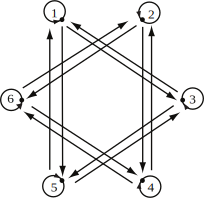
\includegraphics{figps-sec71-dirgraph-b.eps}}
%%\caption{Vertices for $A$} \label{fig:dirgraph3}
%\end{center}
%\end{figure}
\hbreak


\endinput

